% Created by tikzDevice version 0.6.2-92-0ad2792 on 2013-02-06 18:08:00
% !TEX encoding = UTF-8 Unicode
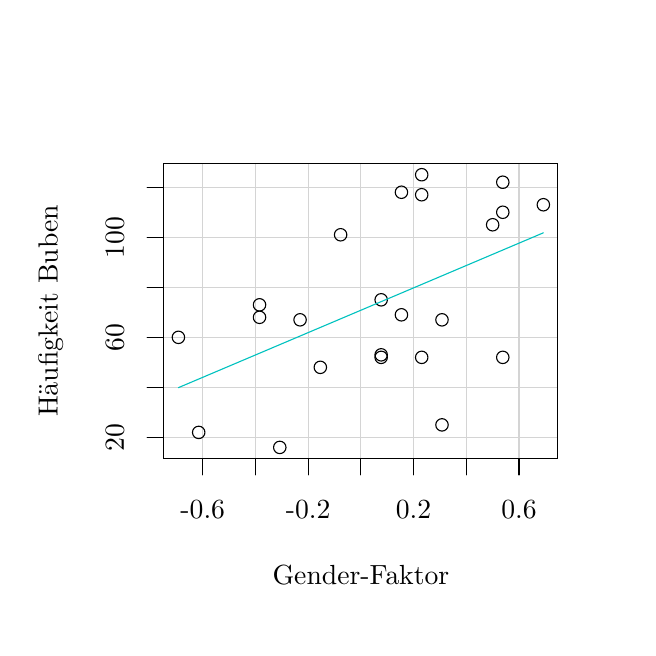
\begin{tikzpicture}[x=1pt,y=1pt]
\definecolor[named]{fillColor}{rgb}{1.00,1.00,1.00}
\path[use as bounding box,fill=fillColor,fill opacity=0.00] (0,0) rectangle (216.81,216.81);
\begin{scope}
\path[clip] (  0.00,  0.00) rectangle (216.81,216.81);
\definecolor[named]{drawColor}{rgb}{0.00,0.00,0.00}

\path[draw=drawColor,line width= 0.4pt,line join=round,line cap=round] ( 63.27, 61.20) -- (177.54, 61.20);

\path[draw=drawColor,line width= 0.4pt,line join=round,line cap=round] ( 63.27, 61.20) -- ( 63.27, 55.20);

\path[draw=drawColor,line width= 0.4pt,line join=round,line cap=round] ( 82.31, 61.20) -- ( 82.31, 55.20);

\path[draw=drawColor,line width= 0.4pt,line join=round,line cap=round] (101.36, 61.20) -- (101.36, 55.20);

\path[draw=drawColor,line width= 0.4pt,line join=round,line cap=round] (120.41, 61.20) -- (120.41, 55.20);

\path[draw=drawColor,line width= 0.4pt,line join=round,line cap=round] (139.45, 61.20) -- (139.45, 55.20);

\path[draw=drawColor,line width= 0.4pt,line join=round,line cap=round] (158.50, 61.20) -- (158.50, 55.20);

\path[draw=drawColor,line width= 0.4pt,line join=round,line cap=round] (177.54, 61.20) -- (177.54, 55.20);

\node[text=drawColor,anchor=base,inner sep=0pt, outer sep=0pt, scale=  1.00] at ( 63.27, 39.60) {-0.6};

\node[text=drawColor,anchor=base,inner sep=0pt, outer sep=0pt, scale=  1.00] at (101.36, 39.60) {-0.2};

\node[text=drawColor,anchor=base,inner sep=0pt, outer sep=0pt, scale=  1.00] at (139.45, 39.60) {0.2};

\node[text=drawColor,anchor=base,inner sep=0pt, outer sep=0pt, scale=  1.00] at (177.54, 39.60) {0.6};

\path[draw=drawColor,line width= 0.4pt,line join=round,line cap=round] ( 49.20, 68.76) -- ( 49.20,159.15);

\path[draw=drawColor,line width= 0.4pt,line join=round,line cap=round] ( 49.20, 68.76) -- ( 43.20, 68.76);

\path[draw=drawColor,line width= 0.4pt,line join=round,line cap=round] ( 49.20, 86.84) -- ( 43.20, 86.84);

\path[draw=drawColor,line width= 0.4pt,line join=round,line cap=round] ( 49.20,104.91) -- ( 43.20,104.91);

\path[draw=drawColor,line width= 0.4pt,line join=round,line cap=round] ( 49.20,122.99) -- ( 43.20,122.99);

\path[draw=drawColor,line width= 0.4pt,line join=round,line cap=round] ( 49.20,141.07) -- ( 43.20,141.07);

\path[draw=drawColor,line width= 0.4pt,line join=round,line cap=round] ( 49.20,159.15) -- ( 43.20,159.15);

\node[text=drawColor,rotate= 90.00,anchor=base,inner sep=0pt, outer sep=0pt, scale=  1.00] at ( 34.80, 68.76) {20};

\node[text=drawColor,rotate= 90.00,anchor=base,inner sep=0pt, outer sep=0pt, scale=  1.00] at ( 34.80,104.91) {60};

\node[text=drawColor,rotate= 90.00,anchor=base,inner sep=0pt, outer sep=0pt, scale=  1.00] at ( 34.80,141.07) {100};

\path[draw=drawColor,line width= 0.4pt,line join=round,line cap=round] ( 49.20, 61.20) --
	(191.61, 61.20) --
	(191.61,167.61) --
	( 49.20,167.61) --
	( 49.20, 61.20);
\end{scope}
\begin{scope}
\path[clip] (  0.00,  0.00) rectangle (216.81,216.81);
\definecolor[named]{drawColor}{rgb}{0.00,0.00,0.00}

\node[text=drawColor,anchor=base,inner sep=0pt, outer sep=0pt, scale=  1.00] at (120.41, 15.60) {Gender-Faktor};

\node[text=drawColor,rotate= 90.00,anchor=base,inner sep=0pt, outer sep=0pt, scale=  1.00] at ( 10.80,114.41) {Häufigkeit Buben};
\end{scope}
\begin{scope}
\path[clip] ( 49.20, 61.20) rectangle (191.61,167.61);
\definecolor[named]{drawColor}{rgb}{0.83,0.83,0.83}

\path[draw=drawColor,line width= 0.4pt,line join=round,line cap=round] ( 63.27, 61.20) -- ( 63.27,167.61);

\path[draw=drawColor,line width= 0.4pt,line join=round,line cap=round] ( 82.31, 61.20) -- ( 82.31,167.61);

\path[draw=drawColor,line width= 0.4pt,line join=round,line cap=round] (101.36, 61.20) -- (101.36,167.61);

\path[draw=drawColor,line width= 0.4pt,line join=round,line cap=round] (120.41, 61.20) -- (120.41,167.61);

\path[draw=drawColor,line width= 0.4pt,line join=round,line cap=round] (139.45, 61.20) -- (139.45,167.61);

\path[draw=drawColor,line width= 0.4pt,line join=round,line cap=round] (158.50, 61.20) -- (158.50,167.61);

\path[draw=drawColor,line width= 0.4pt,line join=round,line cap=round] (177.54, 61.20) -- (177.54,167.61);

\path[draw=drawColor,line width= 0.4pt,line join=round,line cap=round] ( 49.20, 68.76) -- (191.61, 68.76);

\path[draw=drawColor,line width= 0.4pt,line join=round,line cap=round] ( 49.20, 86.84) -- (191.61, 86.84);

\path[draw=drawColor,line width= 0.4pt,line join=round,line cap=round] ( 49.20,104.91) -- (191.61,104.91);

\path[draw=drawColor,line width= 0.4pt,line join=round,line cap=round] ( 49.20,122.99) -- (191.61,122.99);

\path[draw=drawColor,line width= 0.4pt,line join=round,line cap=round] ( 49.20,141.07) -- (191.61,141.07);

\path[draw=drawColor,line width= 0.4pt,line join=round,line cap=round] ( 49.20,159.15) -- (191.61,159.15);
\end{scope}
\begin{scope}
\path[clip] (  0.00,  0.00) rectangle (216.81,216.81);
\definecolor[named]{drawColor}{rgb}{0.00,0.00,0.00}

\path[draw=drawColor,line width= 0.4pt,line join=round,line cap=round] ( 49.20, 61.20) --
	(191.61, 61.20) --
	(191.61,167.61) --
	( 49.20,167.61) --
	( 49.20, 61.20);
\end{scope}
\begin{scope}
\path[clip] ( 49.20, 61.20) rectangle (191.61,167.61);
\definecolor[named]{drawColor}{rgb}{0.00,0.00,0.00}

\path[draw=drawColor,line width= 0.4pt,line join=round,line cap=round] (171.68,150.11) circle (  2.25);

\path[draw=drawColor,line width= 0.4pt,line join=round,line cap=round] (135.06,113.05) circle (  2.25);

\path[draw=drawColor,line width= 0.4pt,line join=round,line cap=round] (149.71,111.24) circle (  2.25);

\path[draw=drawColor,line width= 0.4pt,line join=round,line cap=round] (142.38,156.44) circle (  2.25);

\path[draw=drawColor,line width= 0.4pt,line join=round,line cap=round] (142.38,163.67) circle (  2.25);

\path[draw=drawColor,line width= 0.4pt,line join=round,line cap=round] (171.68,160.96) circle (  2.25);

\path[draw=drawColor,line width= 0.4pt,line join=round,line cap=round] (168.02,145.59) circle (  2.25);

\path[draw=drawColor,line width= 0.4pt,line join=round,line cap=round] (142.38, 97.68) circle (  2.25);

\path[draw=drawColor,line width= 0.4pt,line join=round,line cap=round] (186.34,152.82) circle (  2.25);

\path[draw=drawColor,line width= 0.4pt,line join=round,line cap=round] (127.73, 97.68) circle (  2.25);

\path[draw=drawColor,line width= 0.4pt,line join=round,line cap=round] (113.08,141.97) circle (  2.25);

\path[draw=drawColor,line width= 0.4pt,line join=round,line cap=round] ( 98.43,111.24) circle (  2.25);

\path[draw=drawColor,line width= 0.4pt,line join=round,line cap=round] (135.06,157.34) circle (  2.25);

\path[draw=drawColor,line width= 0.4pt,line join=round,line cap=round] (105.75, 94.07) circle (  2.25);

\path[draw=drawColor,line width= 0.4pt,line join=round,line cap=round] ( 83.78,116.66) circle (  2.25);

\path[draw=drawColor,line width= 0.4pt,line join=round,line cap=round] ( 54.47,104.91) circle (  2.25);

\path[draw=drawColor,line width= 0.4pt,line join=round,line cap=round] ( 83.78,112.15) circle (  2.25);

\path[draw=drawColor,line width= 0.4pt,line join=round,line cap=round] (127.73,118.47) circle (  2.25);

\path[draw=drawColor,line width= 0.4pt,line join=round,line cap=round] (171.68, 97.68) circle (  2.25);

\path[draw=drawColor,line width= 0.4pt,line join=round,line cap=round] (127.73, 98.59) circle (  2.25);

\path[draw=drawColor,line width= 0.4pt,line join=round,line cap=round] (149.71, 73.28) circle (  2.25);

\path[draw=drawColor,line width= 0.4pt,line join=round,line cap=round] ( 91.10, 65.14) circle (  2.25);

\path[draw=drawColor,line width= 0.4pt,line join=round,line cap=round] ( 61.80, 70.56) circle (  2.25);
\definecolor[named]{drawColor}{rgb}{0.00,0.76,0.75}

\path[draw=drawColor,line width= 0.4pt,line join=round,line cap=round] ( 54.47, 86.73) --
	(186.34,142.68);
\end{scope}
\end{tikzpicture}
